\documentclass[conference]{IEEEtran}
\usepackage{amsmath,amssymb}
\usepackage{booktabs}
\usepackage{graphicx}
\usepackage{url}
\usepackage[T1]{fontenc}
\usepackage{microtype}
% generated by paper/p1/make_assets.py -- do not edit
\newcommand{\AucAblIEqAHi}{0.531}
\newcommand{\AucAblIEqALo}{0.234}
\newcommand{\AucAblIEqAMean}{0.383}
\newcommand{\AucAblKmaxOneHi}{0.531}
\newcommand{\AucAblKmaxOneLo}{0.234}
\newcommand{\AucAblKmaxOneMean}{0.383}
\newcommand{\AucAblMmdHi}{0.531}
\newcommand{\AucAblMmdLo}{0.234}
\newcommand{\AucAblMmdMean}{0.383}
\newcommand{\AucAblNoCanaryCtrlHi}{0.531}
\newcommand{\AucAblNoCanaryCtrlLo}{0.234}
\newcommand{\AucAblNoCanaryCtrlMean}{0.383}
\newcommand{\AucAblNoCanaryRealHi}{0.531}
\newcommand{\AucAblNoCanaryRealLo}{0.234}
\newcommand{\AucAblNoCanaryRealMean}{0.383}
\newcommand{\AucAblNoStepSafetyHi}{0.531}
\newcommand{\AucAblNoStepSafetyLo}{0.234}
\newcommand{\AucAblNoStepSafetyMean}{0.383}
\newcommand{\AucAblNoStepTestHi}{0.531}
\newcommand{\AucAblNoStepTestLo}{0.234}
\newcommand{\AucAblNoStepTestMean}{0.383}
\newcommand{\AucAblPooledHi}{0.540}
\newcommand{\AucAblPooledLo}{0.239}
\newcommand{\AucAblPooledMean}{0.389}
\newcommand{\AucAlwaysSmoteHi}{0.534}
\newcommand{\AucAlwaysSmoteLo}{0.235}
\newcommand{\AucAlwaysSmoteMean}{0.384}
\newcommand{\AucCtrlRosHi}{0.531}
\newcommand{\AucCtrlRosLo}{0.234}
\newcommand{\AucCtrlRosMean}{0.383}
\newcommand{\AucCtrlSmoteHi}{0.531}
\newcommand{\AucCtrlSmoteLo}{0.234}
\newcommand{\AucCtrlSmoteMean}{0.383}
\newcommand{\AucCtrlThreshHi}{0.531}
\newcommand{\AucCtrlThreshLo}{0.234}
\newcommand{\AucCtrlThreshMean}{0.383}
\newcommand{\AucFidgateSmoteHi}{0.532}
\newcommand{\AucFidgateSmoteLo}{0.234}
\newcommand{\AucFidgateSmoteMean}{0.383}
\newcommand{\AucFixedSmoteFourHi}{0.532}
\newcommand{\AucFixedSmoteFourLo}{0.234}
\newcommand{\AucFixedSmoteFourMean}{0.383}
\newcommand{\AucFixedSmoteOneHi}{0.533}
\newcommand{\AucFixedSmoteOneLo}{0.235}
\newcommand{\AucFixedSmoteOneMean}{0.384}
\newcommand{\AucFrozenHi}{0.000}
\newcommand{\AucFrozenLo}{0.000}
\newcommand{\AucFrozenMean}{0.000}
\newcommand{\AucNcFourPlaceboDdosHi}{0.531}
\newcommand{\AucNcFourPlaceboDdosLo}{0.234}
\newcommand{\AucNcFourPlaceboDdosMean}{0.383}
\newcommand{\AucNcOneDonorSmoteHi}{0.531}
\newcommand{\AucNcOneDonorSmoteLo}{0.234}
\newcommand{\AucNcOneDonorSmoteMean}{0.383}
\newcommand{\AucNcThreeShuffleHi}{0.531}
\newcommand{\AucNcThreeShuffleLo}{0.234}
\newcommand{\AucNcThreeShuffleMean}{0.383}
\newcommand{\AucNcTwoGaussianHi}{0.531}
\newcommand{\AucNcTwoGaussianLo}{0.234}
\newcommand{\AucNcTwoGaussianMean}{0.383}
\newcommand{\AucOracleDoseHi}{0.000}
\newcommand{\AucOracleDoseLo}{0.000}
\newcommand{\AucOracleDoseMean}{0.000}
\newcommand{\AucRealOnlyAllLabelsHi}{0.485}
\newcommand{\AucRealOnlyAllLabelsLo}{0.056}
\newcommand{\AucRealOnlyAllLabelsMean}{0.270}
\newcommand{\AucRealOnlyHi}{0.531}
\newcommand{\AucRealOnlyLo}{0.234}
\newcommand{\AucRealOnlyMean}{0.383}
\newcommand{\BreachAblIEqA}{0}
\newcommand{\BreachAblKmaxOne}{0}
\newcommand{\BreachAblMmd}{0}
\newcommand{\BreachAblNoCanaryCtrl}{0}
\newcommand{\BreachAblNoCanaryReal}{0}
\newcommand{\BreachAblNoStepSafety}{0}
\newcommand{\BreachAblNoStepTest}{1}
\newcommand{\BreachAblPooled}{0}
\newcommand{\BreachAlwaysSmote}{2}
\newcommand{\BreachCtrlRos}{0}
\newcommand{\BreachCtrlSmote}{0}
\newcommand{\BreachCtrlThresh}{0}
\newcommand{\BreachFidgateSmote}{0}
\newcommand{\BreachFixedSmoteFour}{1}
\newcommand{\BreachFixedSmoteOne}{2}
\newcommand{\BreachFrozen}{0}
\newcommand{\BreachNcFourPlaceboDdos}{0}
\newcommand{\BreachNcOneDonorSmote}{0}
\newcommand{\BreachNcThreeShuffle}{0}
\newcommand{\BreachNcTwoGaussian}{0}
\newcommand{\BreachOracleDose}{0}
\newcommand{\BreachRealOnly}{0}
\newcommand{\BreachRealOnlyAllLabels}{4}
\newcommand{\CandCtrlRos}{59}
\newcommand{\CandCtrlSmote}{59}
\newcommand{\CandCtrlThresh}{59}
\newcommand{\CandMaxLcbCtrlRos}{0.000}
\newcommand{\CandMaxLcbCtrlSmote}{0.000}
\newcommand{\CandMaxLcbCtrlThresh}{0.012}
\newcommand{\CandMaxPtCtrlRos}{0.044}
\newcommand{\CandMaxPtCtrlSmote}{0.070}
\newcommand{\CandMaxPtCtrlThresh}{0.076}
\newcommand{\CandMedRowsCtrlRos}{48}
\newcommand{\CandMedRowsCtrlSmote}{48}
\newcommand{\CandPosCtrlRos}{14}
\newcommand{\CandPosCtrlSmote}{21}
\newcommand{\CandPosCtrlThresh}{44}
\newcommand{\ChkAblIEqA}{14}
\newcommand{\ChkAblKmaxOne}{14}
\newcommand{\ChkAblMmd}{14}
\newcommand{\ChkAblNoCanaryCtrl}{0}
\newcommand{\ChkAblNoCanaryReal}{0}
\newcommand{\ChkAblNoStepSafety}{14}
\newcommand{\ChkAblNoStepTest}{14}
\newcommand{\ChkAblPooled}{17}
\newcommand{\ChkAlwaysSmote}{15}
\newcommand{\ChkCtrlRos}{14}
\newcommand{\ChkCtrlSmote}{14}
\newcommand{\ChkCtrlThresh}{14}
\newcommand{\ChkFidgateSmote}{14}
\newcommand{\ChkFixedSmoteFour}{14}
\newcommand{\ChkFixedSmoteOne}{15}
\newcommand{\ChkFrozen}{0}
\newcommand{\ChkNcFourPlaceboDdos}{14}
\newcommand{\ChkNcOneDonorSmote}{14}
\newcommand{\ChkNcThreeShuffle}{14}
\newcommand{\ChkNcTwoGaussian}{14}
\newcommand{\ChkOracleDose}{0}
\newcommand{\ChkRealOnly}{14}
\newcommand{\ChkRealOnlyAllLabels}{5}
\newcommand{\DepDiffAblPooledHi}{0.0090}
\newcommand{\DepDiffAblPooledLo}{-0.0000}
\newcommand{\DepDiffAblPooledMean}{0.0045}
\newcommand{\DepDiffAlwaysSmoteHi}{0.0016}
\newcommand{\DepDiffAlwaysSmoteLo}{-0.0009}
\newcommand{\DepDiffAlwaysSmoteMean}{0.0003}
\newcommand{\DepDiffFidgateSmoteHi}{0.0025}
\newcommand{\DepDiffFidgateSmoteLo}{-0.0010}
\newcommand{\DepDiffFidgateSmoteMean}{0.0008}
\newcommand{\DepDiffFixedSmoteFourHi}{0.0038}
\newcommand{\DepDiffFixedSmoteFourLo}{-0.0015}
\newcommand{\DepDiffFixedSmoteFourMean}{0.0012}
\newcommand{\DepDiffFixedSmoteOneHi}{0.0017}
\newcommand{\DepDiffFixedSmoteOneLo}{-0.0021}
\newcommand{\DepDiffFixedSmoteOneMean}{-0.0002}
\newcommand{\DepDiffRealOnlyAllLabelsHi}{0.2297}
\newcommand{\DepDiffRealOnlyAllLabelsLo}{-0.7320}
\newcommand{\DepDiffRealOnlyAllLabelsMean}{-0.2511}
\newcommand{\FitsAblIEqA}{131}
\newcommand{\FitsAblKmaxOne}{59}
\newcommand{\FitsAblMmd}{59}
\newcommand{\FitsAblNoCanaryCtrl}{59}
\newcommand{\FitsAblNoCanaryReal}{0}
\newcommand{\FitsAblNoStepSafety}{59}
\newcommand{\FitsAblNoStepTest}{69}
\newcommand{\FitsAblPooled}{87}
\newcommand{\FitsAlwaysSmote}{0}
\newcommand{\FitsCtrlRos}{59}
\newcommand{\FitsCtrlSmote}{59}
\newcommand{\FitsCtrlThresh}{59}
\newcommand{\FitsFidgateSmote}{0}
\newcommand{\FitsFixedSmoteFour}{0}
\newcommand{\FitsFixedSmoteOne}{0}
\newcommand{\FitsFrozen}{0}
\newcommand{\FitsNcFourPlaceboDdos}{0}
\newcommand{\FitsNcOneDonorSmote}{59}
\newcommand{\FitsNcThreeShuffle}{59}
\newcommand{\FitsNcTwoGaussian}{59}
\newcommand{\FitsOracleDose}{0}
\newcommand{\FitsRealOnly}{0}
\newcommand{\FitsRealOnlyAllLabels}{0}
\newcommand{\FlagFEight}{fired}
\newcommand{\FlagFFive}{not fired}
\newcommand{\FlagFFour}{not fired}
\newcommand{\FlagFNine}{not fired}
\newcommand{\FlagFOneOne}{not fired}
\newcommand{\FlagFOneZero}{not fired}
\newcommand{\FlagFThreeA}{fired}
\newcommand{\FlagFThreeB}{fired}
\newcommand{\FlagFTwo}{fired}
\newcommand{\HThreeAHi}{0.000}
\newcommand{\HThreeALo}{0.000}
\newcommand{\HThreeAMean}{0.000}
\newcommand{\HThreeARejected}{not rejected}
\newcommand{\HThreeBHi}{0.000}
\newcommand{\HThreeBLo}{0.000}
\newcommand{\HThreeBMean}{0.000}
\newcommand{\HThreeBRejected}{not rejected}
\newcommand{\HTwoHi}{0.000}
\newcommand{\HTwoLo}{0.000}
\newcommand{\HTwoMean}{0.000}
\newcommand{\HTwoRejected}{not rejected}
\newcommand{\HfiveFixedSmoteFourHi}{0.001}
\newcommand{\HfiveFixedSmoteFourLo}{-0.004}
\newcommand{\HfiveFixedSmoteFourMean}{-0.001}
\newcommand{\HfiveFixedSmoteOneHi}{0.002}
\newcommand{\HfiveFixedSmoteOneLo}{-0.002}
\newcommand{\HfiveFixedSmoteOneMean}{0.000}
\newcommand{\NAblIEqAEnvelopeInconclusive}{26}
\newcommand{\NAblIEqANoAffectedRegion}{14}
\newcommand{\NAblIEqAPromoted}{14}
\newcommand{\NAblIEqAUtilityInconclusive}{20}
\newcommand{\NAblIEqAUtilityNoGain}{16}
\newcommand{\NAblKmaxOneEnvelopeInconclusive}{26}
\newcommand{\NAblKmaxOneNoAffectedRegion}{14}
\newcommand{\NAblKmaxOnePromoted}{14}
\newcommand{\NAblKmaxOneUtilityInconclusive}{20}
\newcommand{\NAblKmaxOneUtilityNoGain}{16}
\newcommand{\NAblMmdEnvelopeInconclusive}{26}
\newcommand{\NAblMmdNoAffectedRegion}{14}
\newcommand{\NAblMmdPromoted}{14}
\newcommand{\NAblMmdUtilityInconclusive}{20}
\newcommand{\NAblMmdUtilityNoGain}{16}
\newcommand{\NAblNoCanaryCtrlEnvelopeInconclusive}{26}
\newcommand{\NAblNoCanaryCtrlNoAffectedRegion}{14}
\newcommand{\NAblNoCanaryCtrlPromoted}{14}
\newcommand{\NAblNoCanaryCtrlUtilityInconclusive}{20}
\newcommand{\NAblNoCanaryCtrlUtilityNoGain}{16}
\newcommand{\NAblNoCanaryRealEnvelopeInconclusive}{26}
\newcommand{\NAblNoCanaryRealNoAffectedRegion}{14}
\newcommand{\NAblNoCanaryRealPromoted}{14}
\newcommand{\NAblNoCanaryRealUtilityInconclusive}{20}
\newcommand{\NAblNoCanaryRealUtilityNoGain}{16}
\newcommand{\NAblNoStepSafetyEnvelopeInconclusive}{26}
\newcommand{\NAblNoStepSafetyNoAffectedRegion}{14}
\newcommand{\NAblNoStepSafetyPromoted}{14}
\newcommand{\NAblNoStepSafetyUtilityInconclusive}{20}
\newcommand{\NAblNoStepSafetyUtilityNoGain}{16}
\newcommand{\NAblNoStepTestEnvelopeInconclusive}{26}
\newcommand{\NAblNoStepTestNoAffectedRegion}{14}
\newcommand{\NAblNoStepTestPromoted}{15}
\newcommand{\NAblNoStepTestUtilityInconclusive}{19}
\newcommand{\NAblNoStepTestUtilityNoGain}{16}
\newcommand{\NAblPooledEnvelopeInconclusive}{35}
\newcommand{\NAblPooledNoAffectedRegion}{2}
\newcommand{\NAblPooledPromoted}{17}
\newcommand{\NAblPooledUtilityInconclusive}{25}
\newcommand{\NAblPooledUtilityNoGain}{11}
\newcommand{\NAlwaysSmoteEnvelopeInconclusive}{26}
\newcommand{\NAlwaysSmoteNoAffectedRegion}{12}
\newcommand{\NAlwaysSmotePromoted}{15}
\newcommand{\NAlwaysSmoteUtilityInconclusive}{18}
\newcommand{\NAlwaysSmoteUtilityNoGain}{19}
\newcommand{\NCtrlRosEnvelopeInconclusive}{26}
\newcommand{\NCtrlRosNoAffectedRegion}{14}
\newcommand{\NCtrlRosPromoted}{14}
\newcommand{\NCtrlRosUtilityInconclusive}{20}
\newcommand{\NCtrlRosUtilityNoGain}{16}
\newcommand{\NCtrlSmoteEnvelopeInconclusive}{26}
\newcommand{\NCtrlSmoteNoAffectedRegion}{14}
\newcommand{\NCtrlSmotePromoted}{14}
\newcommand{\NCtrlSmoteUtilityInconclusive}{20}
\newcommand{\NCtrlSmoteUtilityNoGain}{16}
\newcommand{\NCtrlThreshEnvelopeInconclusive}{26}
\newcommand{\NCtrlThreshNoAffectedRegion}{14}
\newcommand{\NCtrlThreshPromoted}{14}
\newcommand{\NCtrlThreshUtilityInconclusive}{20}
\newcommand{\NCtrlThreshUtilityNoGain}{16}
\newcommand{\NFidgateSmoteEnvelopeInconclusive}{26}
\newcommand{\NFidgateSmoteNoAffectedRegion}{11}
\newcommand{\NFidgateSmotePromoted}{15}
\newcommand{\NFidgateSmoteUtilityInconclusive}{20}
\newcommand{\NFidgateSmoteUtilityNoGain}{18}
\newcommand{\NFixedSmoteFourEnvelopeInconclusive}{26}
\newcommand{\NFixedSmoteFourNoAffectedRegion}{11}
\newcommand{\NFixedSmoteFourPromoted}{16}
\newcommand{\NFixedSmoteFourUtilityInconclusive}{19}
\newcommand{\NFixedSmoteFourUtilityNoGain}{18}
\newcommand{\NFixedSmoteOneEnvelopeInconclusive}{26}
\newcommand{\NFixedSmoteOneNoAffectedRegion}{11}
\newcommand{\NFixedSmoteOnePromoted}{15}
\newcommand{\NFixedSmoteOneUtilityInconclusive}{19}
\newcommand{\NFixedSmoteOneUtilityNoGain}{19}
\newcommand{\NFrozenFrozen}{90}
\newcommand{\NNcFourPlaceboDdosEnvelopeInconclusive}{26}
\newcommand{\NNcFourPlaceboDdosNoAffectedRegion}{14}
\newcommand{\NNcFourPlaceboDdosPromoted}{14}
\newcommand{\NNcFourPlaceboDdosUtilityInconclusive}{20}
\newcommand{\NNcFourPlaceboDdosUtilityNoGain}{16}
\newcommand{\NNcOneDonorSmoteEnvelopeInconclusive}{26}
\newcommand{\NNcOneDonorSmoteNoAffectedRegion}{14}
\newcommand{\NNcOneDonorSmotePromoted}{14}
\newcommand{\NNcOneDonorSmoteUtilityInconclusive}{20}
\newcommand{\NNcOneDonorSmoteUtilityNoGain}{16}
\newcommand{\NNcThreeShuffleEnvelopeInconclusive}{26}
\newcommand{\NNcThreeShuffleNoAffectedRegion}{14}
\newcommand{\NNcThreeShufflePromoted}{14}
\newcommand{\NNcThreeShuffleUtilityInconclusive}{20}
\newcommand{\NNcThreeShuffleUtilityNoGain}{16}
\newcommand{\NNcTwoGaussianEnvelopeInconclusive}{26}
\newcommand{\NNcTwoGaussianNoAffectedRegion}{14}
\newcommand{\NNcTwoGaussianPromoted}{14}
\newcommand{\NNcTwoGaussianUtilityInconclusive}{20}
\newcommand{\NNcTwoGaussianUtilityNoGain}{16}
\newcommand{\NOracleDoseReferenceNotDeployed}{90}
\newcommand{\NRealOnlyAllLabelsEnvelopeInconclusive}{67}
\newcommand{\NRealOnlyAllLabelsEnvelopeViolated}{2}
\newcommand{\NRealOnlyAllLabelsNoAffectedRegion}{1}
\newcommand{\NRealOnlyAllLabelsPromoted}{5}
\newcommand{\NRealOnlyAllLabelsUtilityInconclusive}{13}
\newcommand{\NRealOnlyAllLabelsUtilityNoGain}{2}
\newcommand{\NRealOnlyEnvelopeInconclusive}{26}
\newcommand{\NRealOnlyNoAffectedRegion}{14}
\newcommand{\NRealOnlyPromoted}{14}
\newcommand{\NRealOnlyUtilityInconclusive}{20}
\newcommand{\NRealOnlyUtilityNoGain}{16}
\newcommand{\NonBaseAblIEqA}{71}
\newcommand{\NonBaseAblKmaxOne}{71}
\newcommand{\NonBaseAblMmd}{71}
\newcommand{\NonBaseAblNoCanaryCtrl}{71}
\newcommand{\NonBaseAblNoCanaryReal}{71}
\newcommand{\NonBaseAblNoStepSafety}{71}
\newcommand{\NonBaseAblNoStepTest}{71}
\newcommand{\NonBaseAblPooled}{71}
\newcommand{\NonBaseAlwaysSmote}{71}
\newcommand{\NonBaseCtrlRos}{71}
\newcommand{\NonBaseCtrlSmote}{71}
\newcommand{\NonBaseCtrlThresh}{71}
\newcommand{\NonBaseFidgateSmote}{71}
\newcommand{\NonBaseFixedSmoteFour}{71}
\newcommand{\NonBaseFixedSmoteOne}{71}
\newcommand{\NonBaseFrozen}{0}
\newcommand{\NonBaseNcFourPlaceboDdos}{71}
\newcommand{\NonBaseNcOneDonorSmote}{71}
\newcommand{\NonBaseNcThreeShuffle}{71}
\newcommand{\NonBaseNcTwoGaussian}{71}
\newcommand{\NonBaseOracleDose}{0}
\newcommand{\NonBaseRealOnly}{71}
\newcommand{\NonBaseRealOnlyAllLabels}{40}
\newcommand{\RealAblIEqA}{14}
\newcommand{\RealAblKmaxOne}{14}
\newcommand{\RealAblMmd}{14}
\newcommand{\RealAblNoCanaryCtrl}{14}
\newcommand{\RealAblNoCanaryReal}{14}
\newcommand{\RealAblNoStepSafety}{14}
\newcommand{\RealAblNoStepTest}{14}
\newcommand{\RealAblPooled}{17}
\newcommand{\RealAlwaysSmote}{13}
\newcommand{\RealCtrlRos}{14}
\newcommand{\RealCtrlSmote}{14}
\newcommand{\RealCtrlThresh}{14}
\newcommand{\RealFidgateSmote}{13}
\newcommand{\RealFixedSmoteFour}{13}
\newcommand{\RealFixedSmoteOne}{13}
\newcommand{\RealFrozen}{0}
\newcommand{\RealNcFourPlaceboDdos}{14}
\newcommand{\RealNcOneDonorSmote}{14}
\newcommand{\RealNcThreeShuffle}{14}
\newcommand{\RealNcTwoGaussian}{14}
\newcommand{\RealOracleDose}{0}
\newcommand{\RealRealOnly}{14}
\newcommand{\RealRealOnlyAllLabels}{5}
\newcommand{\RmAblIEqAHi}{0.967}
\newcommand{\RmAblIEqALo}{0.436}
\newcommand{\RmAblIEqAMean}{0.701}
\newcommand{\RmAblKmaxOneHi}{0.967}
\newcommand{\RmAblKmaxOneLo}{0.436}
\newcommand{\RmAblKmaxOneMean}{0.701}
\newcommand{\RmAblMmdHi}{0.967}
\newcommand{\RmAblMmdLo}{0.436}
\newcommand{\RmAblMmdMean}{0.701}
\newcommand{\RmAblNoCanaryCtrlHi}{0.967}
\newcommand{\RmAblNoCanaryCtrlLo}{0.436}
\newcommand{\RmAblNoCanaryCtrlMean}{0.701}
\newcommand{\RmAblNoCanaryRealHi}{0.967}
\newcommand{\RmAblNoCanaryRealLo}{0.436}
\newcommand{\RmAblNoCanaryRealMean}{0.701}
\newcommand{\RmAblNoStepSafetyHi}{0.967}
\newcommand{\RmAblNoStepSafetyLo}{0.436}
\newcommand{\RmAblNoStepSafetyMean}{0.701}
\newcommand{\RmAblNoStepTestHi}{0.967}
\newcommand{\RmAblNoStepTestLo}{0.436}
\newcommand{\RmAblNoStepTestMean}{0.701}
\newcommand{\RmAblPooledHi}{0.974}
\newcommand{\RmAblPooledLo}{0.439}
\newcommand{\RmAblPooledMean}{0.706}
\newcommand{\RmAlwaysSmoteHi}{0.967}
\newcommand{\RmAlwaysSmoteLo}{0.436}
\newcommand{\RmAlwaysSmoteMean}{0.702}
\newcommand{\RmCtrlRosHi}{0.967}
\newcommand{\RmCtrlRosLo}{0.436}
\newcommand{\RmCtrlRosMean}{0.701}
\newcommand{\RmCtrlSmoteHi}{0.967}
\newcommand{\RmCtrlSmoteLo}{0.436}
\newcommand{\RmCtrlSmoteMean}{0.701}
\newcommand{\RmCtrlThreshHi}{0.967}
\newcommand{\RmCtrlThreshLo}{0.436}
\newcommand{\RmCtrlThreshMean}{0.701}
\newcommand{\RmFidgateSmoteHi}{0.968}
\newcommand{\RmFidgateSmoteLo}{0.436}
\newcommand{\RmFidgateSmoteMean}{0.702}
\newcommand{\RmFixedSmoteFourHi}{0.969}
\newcommand{\RmFixedSmoteFourLo}{0.436}
\newcommand{\RmFixedSmoteFourMean}{0.703}
\newcommand{\RmFixedSmoteOneHi}{0.967}
\newcommand{\RmFixedSmoteOneLo}{0.436}
\newcommand{\RmFixedSmoteOneMean}{0.701}
\newcommand{\RmFrozenHi}{0.000}
\newcommand{\RmFrozenLo}{0.000}
\newcommand{\RmFrozenMean}{0.000}
\newcommand{\RmNcFourPlaceboDdosHi}{0.967}
\newcommand{\RmNcFourPlaceboDdosLo}{0.436}
\newcommand{\RmNcFourPlaceboDdosMean}{0.701}
\newcommand{\RmNcOneDonorSmoteHi}{0.967}
\newcommand{\RmNcOneDonorSmoteLo}{0.436}
\newcommand{\RmNcOneDonorSmoteMean}{0.701}
\newcommand{\RmNcThreeShuffleHi}{0.967}
\newcommand{\RmNcThreeShuffleLo}{0.436}
\newcommand{\RmNcThreeShuffleMean}{0.701}
\newcommand{\RmNcTwoGaussianHi}{0.967}
\newcommand{\RmNcTwoGaussianLo}{0.436}
\newcommand{\RmNcTwoGaussianMean}{0.701}
\newcommand{\RmOracleDoseHi}{0.000}
\newcommand{\RmOracleDoseLo}{0.000}
\newcommand{\RmOracleDoseMean}{0.000}
\newcommand{\RmRealOnlyAllLabelsHi}{0.758}
\newcommand{\RmRealOnlyAllLabelsLo}{0.079}
\newcommand{\RmRealOnlyAllLabelsMean}{0.419}
\newcommand{\RmRealOnlyHi}{0.967}
\newcommand{\RmRealOnlyLo}{0.436}
\newcommand{\RmRealOnlyMean}{0.701}
\newcommand{\RollAblIEqA}{0}
\newcommand{\RollAblKmaxOne}{0}
\newcommand{\RollAblMmd}{0}
\newcommand{\RollAblNoCanaryCtrl}{0}
\newcommand{\RollAblNoCanaryReal}{0}
\newcommand{\RollAblNoStepSafety}{0}
\newcommand{\RollAblNoStepTest}{0}
\newcommand{\RollAblPooled}{0}
\newcommand{\RollAlwaysSmote}{0}
\newcommand{\RollCtrlRos}{0}
\newcommand{\RollCtrlSmote}{0}
\newcommand{\RollCtrlThresh}{0}
\newcommand{\RollFidgateSmote}{0}
\newcommand{\RollFixedSmoteFour}{0}
\newcommand{\RollFixedSmoteOne}{0}
\newcommand{\RollFrozen}{0}
\newcommand{\RollNcFourPlaceboDdos}{0}
\newcommand{\RollNcOneDonorSmote}{0}
\newcommand{\RollNcThreeShuffle}{0}
\newcommand{\RollNcTwoGaussian}{0}
\newcommand{\RollOracleDose}{0}
\newcommand{\RollRealOnly}{0}
\newcommand{\RollRealOnlyAllLabels}{0}
\newcommand{\RrAblIEqAHi}{0.859}
\newcommand{\RrAblIEqALo}{0.387}
\newcommand{\RrAblIEqAMean}{0.623}
\newcommand{\RrAblKmaxOneHi}{0.859}
\newcommand{\RrAblKmaxOneLo}{0.387}
\newcommand{\RrAblKmaxOneMean}{0.623}
\newcommand{\RrAblMmdHi}{0.859}
\newcommand{\RrAblMmdLo}{0.387}
\newcommand{\RrAblMmdMean}{0.623}
\newcommand{\RrAblNoCanaryCtrlHi}{0.859}
\newcommand{\RrAblNoCanaryCtrlLo}{0.387}
\newcommand{\RrAblNoCanaryCtrlMean}{0.623}
\newcommand{\RrAblNoCanaryRealHi}{0.859}
\newcommand{\RrAblNoCanaryRealLo}{0.387}
\newcommand{\RrAblNoCanaryRealMean}{0.623}
\newcommand{\RrAblNoStepSafetyHi}{0.859}
\newcommand{\RrAblNoStepSafetyLo}{0.387}
\newcommand{\RrAblNoStepSafetyMean}{0.623}
\newcommand{\RrAblNoStepTestHi}{0.859}
\newcommand{\RrAblNoStepTestLo}{0.387}
\newcommand{\RrAblNoStepTestMean}{0.623}
\newcommand{\RrAblPooledHi}{0.866}
\newcommand{\RrAblPooledLo}{0.390}
\newcommand{\RrAblPooledMean}{0.628}
\newcommand{\RrAlwaysSmoteHi}{0.860}
\newcommand{\RrAlwaysSmoteLo}{0.387}
\newcommand{\RrAlwaysSmoteMean}{0.624}
\newcommand{\RrCtrlRosHi}{0.859}
\newcommand{\RrCtrlRosLo}{0.387}
\newcommand{\RrCtrlRosMean}{0.623}
\newcommand{\RrCtrlSmoteHi}{0.859}
\newcommand{\RrCtrlSmoteLo}{0.387}
\newcommand{\RrCtrlSmoteMean}{0.623}
\newcommand{\RrCtrlThreshHi}{0.859}
\newcommand{\RrCtrlThreshLo}{0.387}
\newcommand{\RrCtrlThreshMean}{0.623}
\newcommand{\RrFidgateSmoteHi}{0.861}
\newcommand{\RrFidgateSmoteLo}{0.388}
\newcommand{\RrFidgateSmoteMean}{0.624}
\newcommand{\RrFixedSmoteFourHi}{0.861}
\newcommand{\RrFixedSmoteFourLo}{0.388}
\newcommand{\RrFixedSmoteFourMean}{0.625}
\newcommand{\RrFixedSmoteOneHi}{0.859}
\newcommand{\RrFixedSmoteOneLo}{0.387}
\newcommand{\RrFixedSmoteOneMean}{0.623}
\newcommand{\RrFrozenHi}{0.000}
\newcommand{\RrFrozenLo}{0.000}
\newcommand{\RrFrozenMean}{0.000}
\newcommand{\RrNcFourPlaceboDdosHi}{0.859}
\newcommand{\RrNcFourPlaceboDdosLo}{0.387}
\newcommand{\RrNcFourPlaceboDdosMean}{0.623}
\newcommand{\RrNcOneDonorSmoteHi}{0.859}
\newcommand{\RrNcOneDonorSmoteLo}{0.387}
\newcommand{\RrNcOneDonorSmoteMean}{0.623}
\newcommand{\RrNcThreeShuffleHi}{0.859}
\newcommand{\RrNcThreeShuffleLo}{0.387}
\newcommand{\RrNcThreeShuffleMean}{0.623}
\newcommand{\RrNcTwoGaussianHi}{0.859}
\newcommand{\RrNcTwoGaussianLo}{0.387}
\newcommand{\RrNcTwoGaussianMean}{0.623}
\newcommand{\RrOracleDoseHi}{0.000}
\newcommand{\RrOracleDoseLo}{0.000}
\newcommand{\RrOracleDoseMean}{0.000}
\newcommand{\RrRealOnlyAllLabelsHi}{0.674}
\newcommand{\RrRealOnlyAllLabelsLo}{0.070}
\newcommand{\RrRealOnlyAllLabelsMean}{0.372}
\newcommand{\RrRealOnlyHi}{0.859}
\newcommand{\RrRealOnlyLo}{0.387}
\newcommand{\RrRealOnlyMean}{0.623}
\newcommand{\SeedsAblIEqA}{0}
\newcommand{\SeedsAblKmaxOne}{0}
\newcommand{\SeedsAblMmd}{0}
\newcommand{\SeedsAblNoCanaryCtrl}{0}
\newcommand{\SeedsAblNoCanaryReal}{0}
\newcommand{\SeedsAblNoStepSafety}{0}
\newcommand{\SeedsAblNoStepTest}{1}
\newcommand{\SeedsAblPooled}{0}
\newcommand{\SeedsAlwaysSmote}{2}
\newcommand{\SeedsCtrlRos}{0}
\newcommand{\SeedsCtrlSmote}{0}
\newcommand{\SeedsCtrlThresh}{0}
\newcommand{\SeedsFidgateSmote}{2}
\newcommand{\SeedsFixedSmoteFour}{3}
\newcommand{\SeedsFixedSmoteOne}{2}
\newcommand{\SeedsFrozen}{0}
\newcommand{\SeedsNcFourPlaceboDdos}{0}
\newcommand{\SeedsNcOneDonorSmote}{0}
\newcommand{\SeedsNcThreeShuffle}{0}
\newcommand{\SeedsNcTwoGaussian}{0}
\newcommand{\SeedsOracleDose}{0}
\newcommand{\SeedsRealOnly}{0}
\newcommand{\SeedsRealOnlyAllLabels}{0}
\newcommand{\ShAblIEqAHi}{0.928}
\newcommand{\ShAblIEqALo}{0.895}
\newcommand{\ShAblIEqAMean}{0.911}
\newcommand{\ShAblKmaxOneHi}{0.928}
\newcommand{\ShAblKmaxOneLo}{0.895}
\newcommand{\ShAblKmaxOneMean}{0.911}
\newcommand{\ShAblMmdHi}{0.928}
\newcommand{\ShAblMmdLo}{0.895}
\newcommand{\ShAblMmdMean}{0.911}
\newcommand{\ShAblNoCanaryCtrlHi}{0.928}
\newcommand{\ShAblNoCanaryCtrlLo}{0.895}
\newcommand{\ShAblNoCanaryCtrlMean}{0.911}
\newcommand{\ShAblNoCanaryRealHi}{0.928}
\newcommand{\ShAblNoCanaryRealLo}{0.895}
\newcommand{\ShAblNoCanaryRealMean}{0.911}
\newcommand{\ShAblNoStepSafetyHi}{0.928}
\newcommand{\ShAblNoStepSafetyLo}{0.895}
\newcommand{\ShAblNoStepSafetyMean}{0.911}
\newcommand{\ShAblNoStepTestHi}{0.928}
\newcommand{\ShAblNoStepTestLo}{0.895}
\newcommand{\ShAblNoStepTestMean}{0.911}
\newcommand{\ShAblPooledHi}{0.930}
\newcommand{\ShAblPooledLo}{0.896}
\newcommand{\ShAblPooledMean}{0.913}
\newcommand{\ShAlwaysSmoteHi}{0.933}
\newcommand{\ShAlwaysSmoteLo}{0.898}
\newcommand{\ShAlwaysSmoteMean}{0.916}
\newcommand{\ShCtrlRosHi}{0.928}
\newcommand{\ShCtrlRosLo}{0.895}
\newcommand{\ShCtrlRosMean}{0.911}
\newcommand{\ShCtrlSmoteHi}{0.928}
\newcommand{\ShCtrlSmoteLo}{0.895}
\newcommand{\ShCtrlSmoteMean}{0.911}
\newcommand{\ShCtrlThreshHi}{0.928}
\newcommand{\ShCtrlThreshLo}{0.895}
\newcommand{\ShCtrlThreshMean}{0.911}
\newcommand{\ShDiffAblPooledHi}{0.0050}
\newcommand{\ShDiffAblPooledLo}{-0.0008}
\newcommand{\ShDiffAblPooledMean}{0.0021}
\newcommand{\ShDiffAlwaysSmoteHi}{0.0063}
\newcommand{\ShDiffAlwaysSmoteLo}{0.0029}
\newcommand{\ShDiffAlwaysSmoteMean}{0.0046}
\newcommand{\ShDiffFidgateSmoteHi}{0.0115}
\newcommand{\ShDiffFidgateSmoteLo}{0.0058}
\newcommand{\ShDiffFidgateSmoteMean}{0.0087}
\newcommand{\ShDiffFixedSmoteFourHi}{0.0119}
\newcommand{\ShDiffFixedSmoteFourLo}{0.0058}
\newcommand{\ShDiffFixedSmoteFourMean}{0.0089}
\newcommand{\ShDiffFixedSmoteOneHi}{0.0054}
\newcommand{\ShDiffFixedSmoteOneLo}{0.0020}
\newcommand{\ShDiffFixedSmoteOneMean}{0.0037}
\newcommand{\ShDiffOracleDoseHi}{0.0051}
\newcommand{\ShDiffOracleDoseLo}{-0.0007}
\newcommand{\ShDiffOracleDoseMean}{0.0022}
\newcommand{\ShDiffRealOnlyAllLabelsHi}{0.0717}
\newcommand{\ShDiffRealOnlyAllLabelsLo}{0.0536}
\newcommand{\ShDiffRealOnlyAllLabelsMean}{0.0626}
\newcommand{\ShFidgateSmoteHi}{0.937}
\newcommand{\ShFidgateSmoteLo}{0.902}
\newcommand{\ShFidgateSmoteMean}{0.920}
\newcommand{\ShFixedSmoteFourHi}{0.938}
\newcommand{\ShFixedSmoteFourLo}{0.903}
\newcommand{\ShFixedSmoteFourMean}{0.920}
\newcommand{\ShFixedSmoteOneHi}{0.932}
\newcommand{\ShFixedSmoteOneLo}{0.898}
\newcommand{\ShFixedSmoteOneMean}{0.915}
\newcommand{\ShFrozenHi}{0.000}
\newcommand{\ShFrozenLo}{0.000}
\newcommand{\ShFrozenMean}{0.000}
\newcommand{\ShNcFourPlaceboDdosHi}{0.928}
\newcommand{\ShNcFourPlaceboDdosLo}{0.895}
\newcommand{\ShNcFourPlaceboDdosMean}{0.911}
\newcommand{\ShNcOneDonorSmoteHi}{0.928}
\newcommand{\ShNcOneDonorSmoteLo}{0.895}
\newcommand{\ShNcOneDonorSmoteMean}{0.911}
\newcommand{\ShNcThreeShuffleHi}{0.928}
\newcommand{\ShNcThreeShuffleLo}{0.895}
\newcommand{\ShNcThreeShuffleMean}{0.911}
\newcommand{\ShNcTwoGaussianHi}{0.928}
\newcommand{\ShNcTwoGaussianLo}{0.895}
\newcommand{\ShNcTwoGaussianMean}{0.911}
\newcommand{\ShOracleDoseHi}{0.930}
\newcommand{\ShOracleDoseLo}{0.896}
\newcommand{\ShOracleDoseMean}{0.913}
\newcommand{\ShRealOnlyAllLabelsHi}{0.984}
\newcommand{\ShRealOnlyAllLabelsLo}{0.964}
\newcommand{\ShRealOnlyAllLabelsMean}{0.974}
\newcommand{\ShRealOnlyHi}{0.928}
\newcommand{\ShRealOnlyLo}{0.895}
\newcommand{\ShRealOnlyMean}{0.911}
\newcommand{\ShadowDiffHi}{0.000}
\newcommand{\ShadowDiffLo}{0.000}
\newcommand{\ShadowDiffMean}{0.000}
\newcommand{\StarAblIEqA}{0}
\newcommand{\StarAblKmaxOne}{0}
\newcommand{\StarAblMmd}{0}
\newcommand{\StarAblNoCanaryCtrl}{0}
\newcommand{\StarAblNoCanaryReal}{0}
\newcommand{\StarAblNoStepSafety}{0}
\newcommand{\StarAblNoStepTest}{1}
\newcommand{\StarAblPooled}{0}
\newcommand{\StarAlwaysSmote}{2}
\newcommand{\StarCtrlRos}{0}
\newcommand{\StarCtrlSmote}{0}
\newcommand{\StarCtrlThresh}{0}
\newcommand{\StarFidgateSmote}{2}
\newcommand{\StarFixedSmoteFour}{3}
\newcommand{\StarFixedSmoteOne}{2}
\newcommand{\StarFrozen}{0}
\newcommand{\StarNcFourPlaceboDdos}{0}
\newcommand{\StarNcOneDonorSmote}{0}
\newcommand{\StarNcThreeShuffle}{0}
\newcommand{\StarNcTwoGaussian}{0}
\newcommand{\StarOracleDose}{0}
\newcommand{\StarRealOnly}{0}
\newcommand{\StarRealOnlyAllLabels}{0}
\newcommand{\StepAnchorWouldBlockFpr}{0}
\newcommand{\StepAnchorWouldBlockStable}{37}
\newcommand{\StepCandidates}{59}
\newcommand{\StepGainLcbPositive}{0}
\newcommand{\StepSafe}{23}
\newcommand{\WallAblIEqA}{296}
\newcommand{\WallAblKmaxOne}{218}
\newcommand{\WallAblMmd}{267}
\newcommand{\WallAblNoCanaryCtrl}{211}
\newcommand{\WallAblNoCanaryReal}{130}
\newcommand{\WallAblNoStepSafety}{213}
\newcommand{\WallAblNoStepTest}{222}
\newcommand{\WallAblPooled}{269}
\newcommand{\WallAlwaysSmote}{251}
\newcommand{\WallCtrlRos}{212}
\newcommand{\WallCtrlSmote}{214}
\newcommand{\WallCtrlThresh}{152}
\newcommand{\WallFidgateSmote}{274}
\newcommand{\WallFixedSmoteFour}{221}
\newcommand{\WallFixedSmoteOne}{218}
\newcommand{\WallFrozen}{32}
\newcommand{\WallNcFourPlaceboDdos}{233}
\newcommand{\WallNcOneDonorSmote}{232}
\newcommand{\WallNcThreeShuffle}{208}
\newcommand{\WallNcTwoGaussian}{204}
\newcommand{\WallOracleDose}{524}
\newcommand{\WallRealOnly}{133}
\newcommand{\WallRealOnlyAllLabels}{176}
\newcommand{\budget}{100}
\newcommand{\complete}{yes}
\newcommand{\eligibleKzero}{59}
\newcommand{\eligibleRuns}{59}
\newcommand{\gapRealOnly}{0.210}
\newcommand{\gbAllFprCur}{67}
\newcommand{\gbAllFprStable}{56}
\newcommand{\gbAllMedBenign}{2610}
\newcommand{\gbAllRejected}{84}
\newcommand{\gbFprCur}{21}
\newcommand{\gbFprStable}{0}
\newcommand{\gbMedBenign}{130}
\newcommand{\gbOneFp}{0.0077}
\newcommand{\gbRejected}{62}
\newcommand{\gbStableF}{31}
\newcommand{\gbUtil}{36}
\newcommand{\gbUtilOkEnvFail}{26}
\newcommand{\gitSha}{7567ff1}
\newcommand{\goCleanRecall}{0.767}
\newcommand{\hFourBreaches}{0}
\newcommand{\hFourSeeds}{0}
\newcommand{\nArms}{23}
\newcommand{\nGoRows}{21\,077}
\newcommand{\nRows}{2\,100\,021}
\newcommand{\nSeeds}{10}
\newcommand{\pZeroOutcome}{GO}
\newcommand{\pZeroScope}{GO at B=100; NO\_ROOM at B=25}
\newcommand{\prereg}{yes}
\newcommand{\probeNonempty}{0}
\newcommand{\probeWindows}{30}
\newcommand{\recallAll}{0.739}
\newcommand{\recallAmbig}{0.187}
\newcommand{\recallClean}{0.767}
\newcommand{\rulesHash}{d96b03131071ac1a}
\newcommand{\sTwoAssessSeeds}{5}
\newcommand{\sTwoAucBOneZeroZeroFrozen}{0.000}
\newcommand{\sTwoAucBOneZeroZeroRealOnly}{0.192}
\newcommand{\sTwoAucBOneZeroZeroRealOnlyAllLabels}{0.744}
\newcommand{\sTwoAucBTwoFiveFrozen}{0.000}
\newcommand{\sTwoAucBTwoFiveRealOnly}{0.131}
\newcommand{\sTwoAucBTwoFiveRealOnlyAllLabels}{0.744}
\newcommand{\sTwoGoCells}{0}
\newcommand{\sTwoOutcome}{NO\_GO\_NO\_ROOM}
\newcommand{\sTwoR}{DoS GoldenEye, DoS Hulk, DoS Slowhttptest, DoS Slowhttptest - Attempted, DoS slowloris, DoS slowloris - Attempted}
\newcommand{\sTwoScope}{NO\_ROOM at B=25,100}
\newcommand{\sTwoValid}{pass}
\newcommand{\seedsNeverDeployed}{2}
\newcommand{\seedsNeverDeployedList}{0, 5}
\newcommand{\shareAmbig}{4.9}
\newcommand{\specVersion}{1.4}
\newcommand{\totalWallMin}{85}
\newcommand{\verdictBranch}{NEGATIVE: H2 not rejected; fixed sequence stops; P2 (WGAN) cancelled}

\newcommand{\Rrec}{R\mbox{-}recovery}
\newcommand{\thR}{\theta_{R}}
\newcommand{\thb}{\theta_{\mathrm{base}}}
\newcommand{\eps}{\varepsilon}

\begin{document}

\title{Can a Drift-Aware IDS Learn When to Synthesize?\\
A Preregistered Negative Result on Feedback-Controlled Synthetic Intervention}

\author{\IEEEauthorblockN{Adhyan Jain}
\IEEEauthorblockA{Proteus research prototype (local, single machine)\\
Repository: \texttt{github.com/adhyan-jain/Proteus}}}

\maketitle

\begin{abstract}
Drift-aware intrusion detectors are often paired with generative data augmentation, and the gain is usually
reported against a baseline that never sees new labels. We ask a narrower, falsifiable question: after
\emph{real-only} adaptation under a realistic label budget, is there residual per-class deficiency, and can a
sequential controller that adds class-targeted synthetic rows only when their \emph{observed recovery value}
exceeds a cost, inside an explicit safety envelope, beat real-only adaptation, plain duplication, a decision-threshold
shift and fixed-dose augmentation? We build a leak-free, group-disjoint prequential protocol on CICIDS2017
(\nRows{} flows), freeze a feasibility stage (P0: room exists at 100 labels per window, for one ambiguity-qualified
class, PortScan), implement the controller, three generators and controls, a UCB-gated promotion rule and a canary
with rollback, preregister the hypotheses, and run \nArms{} arms over \nSeeds{} paired seeds. The preregistered
test fails: the controller's paired improvement over real-only adaptation is \HTwoMean{} (95\% CI
[\HTwoLo, \HTwoHi]), because at 100 labels per window the selection set cannot certify even the first dose
step (\eligibleKzero{} of \eligibleRuns{} controller runs stop at zero accepted steps). Fixed-dose SMOTE does build
slightly better \emph{candidates} (+\ShDiffFixedSmoteFourMean{} F1, CI [\ShDiffFixedSmoteFourLo, \ShDiffFixedSmoteFourHi]) but this
does not survive deployment (+\DepDiffFixedSmoteFourMean{}, CI [\DepDiffFixedSmoteFourLo, \DepDiffFixedSmoteFourHi]). The dominant
effect is elsewhere: real-only candidates reach R-recovery \ShRealOnlyMean{} on held-out windows but only
\RmRealOnlyMean{} is ever deployed, because the safety gate cannot prove them safe from about a hundred benign
labels. A second scenario (S2) offers no room for intervention at the assessed budgets. We report a negative result about the value of synthetic
data in this regime, a diagnosis (the certification bottleneck), and the protocol and code to test it elsewhere.
We claim no new learning algorithm.
\end{abstract}

\section{Introduction}
Network intrusion detectors degrade when traffic drifts: new attack families appear, and a model trained on
last week's traffic misses them. A popular response couples drift detection with generative augmentation (GANs,
SMOTE-style interpolation) to ``synthesize the missing class''. Most reported gains compare against a frozen
baseline or against an adapter that is given oracle labels for most of every post-drift window. In our own earlier
demonstration the headline $5.91\times$ macro-F1 ratio arose exactly that way, and its own ablation showed real-only adaptation
did as well or better; we therefore treat that number as superseded and not as evidence for synthetic data.

This paper asks the question that comparison skips. \emph{Once a detector adapts on the real labels it actually receives
under a budget, is anything left for synthetic data to repair, and can a controller decide---from measured recovery value,
class-specific need, cost and an explicit safety constraint---when synthetic data is worth adding?} We make the question
operational and falsifiable before running it.

\paragraph*{What this paper contributes}
(1) A leak-free evaluation protocol for drift adaptation under label budgets: group-disjoint partitions by feature-vector
hash, non-replacing windows, one-window label delay, prequential scoring on held-out reporting rows, and a type-level
guarantee that the adaptation code cannot reach them (Section~\ref{sec:protocol}).
(2) A frozen feasibility stage (P0) whose outcome, validity checks and data adequacy are fixed in advance (Section~\ref{sec:p0}).
(3) A controller that selects class and dose by a lower-confidence-bound gain test under an incremental safety filter, a
promotion rule with a fixed-anchor envelope, and a canary with rollback, with controls and ablations (Section~\ref{sec:method}).
(4) A preregistered campaign whose result is negative, plus a diagnosis that separates \emph{candidate quality} from
\emph{certifiability} (Sections~\ref{sec:design}--\ref{sec:results}).
\textbf{Novelty statement.} Every ingredient is known: champion--challenger model updates, high-confidence safety tests
\cite{thomas2015,thomas2019}, SMOTE \cite{chawla2002smote}, bootstrap bounds \cite{efron1979}, fixed-sequence testing
\cite{marcus1976}. We claim no new algorithm. The contribution is the protocol, the preregistered evidence about when this
combination does and does not pay, and the identification of the certification step as the binding constraint.

\section{Related Work}
\textbf{Concept drift} adaptation is surveyed in \cite{gama2014}; we use prequential (test-then-train) evaluation \cite{gama2013}.
\textbf{Class imbalance and augmentation.} Oversampling and synthetic minority generation \cite{chawla2002smote,he2009} and
generative models for flow data \cite{ring2019,gulrajani2017} are standard; fidelity of synthetic batches is often judged by
kernel two-sample statistics \cite{gretton2012}. Our fidelity-gated arm uses a permutation-calibrated MMD pre-filter instead of a
fixed threshold. Threshold shifting as a cost-sensitive alternative to resampling is classical \cite{elkan2001}; we include it as
an explicit baseline because the residual error we observe is recall lost to the benign class.
\textbf{Evaluation hygiene.} Leakage and temporal bias in security ML are documented in \cite{arp2022,pendlebury2019}; the
CICIDS2017 labelling problems that motivated the corrected release we use are in \cite{engelen2021,sharafaldin2018}.
\textbf{Safe model updates.} Promoting a candidate only if a confidence bound on its improvement is positive and a bound on
its harm is within a margin is the logic of high-confidence policy improvement and Seldonian algorithms
\cite{thomas2015,thomas2019}; our gate is an instance of it applied to detector updates.

\section{Problem and Protocol}\label{sec:protocol}
\textbf{Data.} CICIDS2017 (WTMC-2021 corrected release \cite{engelen2021}, \nRows{} rows, 80 features after unification,
25 labels). Scenario~S1 uses Monday--Thursday as the pre-drift pool and Friday as drift (new classes: Bot, DDoS, PortScan and
attempted variants); scenario~S2 uses Monday--Tuesday versus Wednesday (DoS family).

\textbf{Partitions.} Each row has a group id (hash of its feature bytes); \emph{all} partitioning is by group so identical feature
vectors never straddle a boundary. For each seed the pre-drift pool is split into $\mathrm{TRAIN}$ (source of a 20k reference
reservoir $D_{\mathrm{ref}}$), a drift-detector reference, selection and gate sets of stable traffic ($S_{\mathrm{sel}}$, $S_{\mathrm{gate}}$), a reporting set
$S_{\mathrm{report}}$ and pre-drift stream windows. The drift pool is cut into disjoint non-replacing windows $W_t$ of 3000 rows: 30\% reporting rows
$E_t$ (scored, never learned from), and a labelled subset $L_t$ of size $B$ whose rows arrive one window later and are assigned by
group hash to fit ($60\%$), selection ($20\%$) and gate ($20\%$) buffers for good.

\textbf{Prequential order} at window $t$: the deployed model predicts $W_t$ and $E_t$ is scored; the canary may roll back; labels of
window $t-1$ arrive; the controller runs; the chosen model is deployed from $t+1$. The controller receives a single immutable
\texttt{ControllerView} object with fields $D_{\mathrm{ref}},D_{\mathrm{real}},D_{\mathrm{sel}},D_{\mathrm{gate}},S_{\mathrm{sel}},S_{\mathrm{gate}}$ and \emph{no field} for $E_t$, $S_{\mathrm{report}}$ or
future windows; static and runtime tests enforce this.

\textbf{Learner and frozen parameters.} Random forest (100 trees, \texttt{random\_state}=seed), base model
$\thb=\mathrm{fit}(D_{\mathrm{ref}})$ fixed for the whole run. Frozen before any run: $\eps_{\mathrm{def}}{=}0.05$ (deficiency floor), $s_{\min}{=}n_{\min}{=}5$, step cost $\eta{=}0.02$,
non-inferiority margin $0.01$, envelope $\eps_S{=}0.01$ (stable macro-F1 drop) and $\eps_{\mathrm{FPR}}{=}0.005$ (benign false-positive-rate rise),
dose ladder $\rho\in\{0,0.5,1,2,4,8\}$, $M_{\mathrm{cap}}{=}2000$, synthetic share $\le0.5$, $K_{\max}{=}10$, $\alpha{=}0.05$ with $\alpha/2$ at promotion and $\alpha/K_{\max}$ at steps,
and 2000 paired class-stratified bootstrap resamples \cite{efron1979}.

\section{Method}\label{sec:method}
Let $F1_c(\theta;\mathcal D)$ be the one-vs-rest F1 of class $c$ and $\mathrm{LCB}_a,\mathrm{UCB}_a$ the paired bootstrap bounds. At window $t$ with incumbent $\theta_t$:
\begin{enumerate}
\item \textbf{Region.} $A=\{c\in M : \mathrm{LCB}_\alpha(1-F1_c(\theta_t;D_{\mathrm{sel}}))>\eps_{\mathrm{def}}\}$, where $M$ is the set of classes with support $\ge s_{\min}$ in both $D_{\mathrm{sel}}$ and $D_{\mathrm{gate}}$. If $A=\emptyset$ nothing happens.
\item \textbf{Real-only adaptation.} $\thR=\mathrm{fit}(D_{\mathrm{ref}}\cup D_{\mathrm{real}})$ is always built first.
\item \textbf{Need.} $I=\{c\in A:\mathrm{LCB}_\alpha(1-\mathrm{Recall}_c(\thR;D_{\mathrm{sel}}))>\eps_{\mathrm{def}},\ n_c\ge n_{\min}\}$ (recall, not F1: added rows of class $c$ repair $c$'s recall, not other classes' leakage into it).
\item \textbf{Operator.} An operator maps a dose vector $\rho$ to a candidate: for data operators
$\theta(\rho)=\mathrm{fit}(D_{\mathrm{ref}}\cup D_{\mathrm{real}}\cup\bigcup_{c\in I}G_c.\mathrm{sample}(m_c))$, $m_c=\min(\lfloor\rho_c n_c\rfloor,M_{\mathrm{cap}})$ with generators $G_c$ (random duplication, SMOTE) fit \emph{only} on class-$c$ rows of $D_{\mathrm{real}}$; for the threshold operator, $\thR$ with class-score multipliers $\{1,2,4,8,16\}$ followed by argmax (no refit).
\item \textbf{Greedy dose search.} With $U_A(\theta;\mathcal D)=\frac1{|A|}\sum_{c\in A}F1_c(\theta;\mathcal D)$, a step raises one class $c\in I_{\mathrm{active}}$ one rung; its value is
$L_k(c)=\mathrm{LCB}_{\alpha/K_{\max}}\!\big(U_A(\theta_k^{+c};D_{\mathrm{sel}})-U_A(\theta_k;D_{\mathrm{sel}})\big)$. A step is \emph{safe} iff the upper bounds (at $\alpha/K_{\max}$) of the stable macro-F1 drop on $S_{\mathrm{sel}}$, the benign-FPR rise on $S_{\mathrm{sel}}$ and the benign-FPR rise on $D_{\mathrm{sel}}$'s benign rows are $\le\eps_S,\eps_{\mathrm{FPR}},\eps_{\mathrm{FPR}}$ against the \emph{current iterate}. Accept $c^\star=\arg\max L_k$ over safe candidates if $L_k(c^\star)>\eta$; classes that were unsafe or failed leave $I_{\mathrm{active}}$; stop on no admissible action, $k=K_{\max}$, no safe candidate or $L\le\eta$. Risk is a constraint, never a weight.
\item \textbf{Promotion} on $D_{\mathrm{gate}},S_{\mathrm{gate}}$ only, at level $\alpha/2$: the final candidate $\theta^\star$ is promoted iff it passes a sanity check, $\mathrm{LCB}(U_A(\theta^\star)-U_A(\theta_t))>0$, the \emph{anchor-relative} envelope holds ($\mathrm{UCB}\le\eps$ for all three quantities, against the fixed $\thb$ so degradation cannot accumulate over promotions), the point gain over $\thR$ is positive and $\mathrm{LCB}(U_A(\theta^\star)-U_A(\thR))\ge-0.01$. Otherwise $\thR$ goes through the unchanged real-only rule; otherwise the incumbent stays. An envelope check is labelled \emph{violated} only if its lower bound exceeds $\eps$; a failure to prove safety is \emph{inconclusive} and still blocks promotion (fail closed).
\item \textbf{Canary.} Labels arriving after a promotion score the new and previous model; roll back iff $\mathrm{UCB}_\alpha(U_A(\mathrm{new})-U_A(\mathrm{prev}))<0$ or the benign-FPR envelope is established broken.
\end{enumerate}
Every arm shares the learner, partitions, budget and \emph{one} promotion function; arms differ only in how $\theta^\star$ is produced.

\section{Experimental Design}\label{sec:design}
\textbf{P0 (frozen first).} Conditions FROZEN, REAL\_ONLY and an all-labels positive control (REAL\_ONLY\_ALL\_LABELS), scenario S1, budgets $B\in\{25,100\}$, seeds 0--4, oracle trigger. A budget is GO if in $\ge3$ of 5 seeds at least two windows have a repairable class that real-only adaptation still leaves recall-deficient; NO\_ROOM if that was reachable and not reached; UNMEASURABLE otherwise. The repairable set $R$ is the set of drift classes the all-labels control repairs in $\ge3/5$ seeds. Validity checks (leakage, integrity, repairability) can invalidate the run; a null-region diagnostic is reported but never gates.

\textbf{P1 arms} (all through the same gate; 10 seeds 0--9, $B{=}100$, seeds 0--4 on the \emph{same manifests} as P0): FROZEN; REAL\_ONLY; CTRL with duplication, SMOTE or threshold operator; fixed-dose SMOTE ($\rho{=}1,4$ on $I$); always-on SMOTE ($\rho{=}1$ on every class, no need test); fidelity-gated SMOTE ($\rho{=}4$ behind a label-permutation MMD pre-filter); four negative controls (SMOTE on benign rows relabelled as the target, Gaussian rows, per-feature shuffled rows, a placebo dose on DDoS); eight ablations (no step test, $I{:=}A$, no step safety, $K_{\max}{=}1$, MMD pre-filter, pooled selection/gate sets, and no canary for both controller and real-only); references (all labels; an oracle dose scored on the next window, never deployed).

\textbf{Endpoints.} Primary: \emph{\Rrec}, the mean over post-drift windows of the mean E-F1 over the repairable classes ($R$ from P0; not available to any arm) of the \emph{deployed} model on $E_t$. Candidate quality (``shadow''): the same score for the model that \emph{would} have been deployed (the candidate), scored on the next window after the decision. Safety: stable macro-F1 drop and benign-FPR rise of every deployed model on $S_{\mathrm{report}}$.

\textbf{Hypotheses, fixed sequence} (paired per seed, two-sided 95\% $t$-interval over seeds; each test only if the previous rejected its null \cite{marcus1976}): H2 CTRL+SMOTE $-$ REAL\_ONLY; H3a CTRL+SMOTE $-$ CTRL+duplication; H3b CTRL+SMOTE $-$ CTRL+threshold; H5 non-inferiority to fixed-dose SMOTE at the frozen margin. H4 (separate): no deployed CTRL+SMOTE model breaks the $S_{\mathrm{report}}$ envelope \emph{and} synthetic candidates are promoted in $\ge6$ of 10 seeds (else ``safe by inaction''). Reporting conditions F2--F11 (e.g.\ F8: $k{=}0$ in $>80\%$ of controller runs with a need; F9: the GO is explained by contradictory-label rows; F10: better candidates that cannot be certified) were fixed in advance.

\textbf{Gating and freezing.} A learned generator (WGAN-GP, pretrained on $D_{\mathrm{ref}}$ only) runs only if H2, H3a and H3b all reject; scenario~S2 is run only through its own P0 gate under the unchanged rules, and the P1 arms run on S2 only if that gate is GO. The normative preregistration text is hashed (SHA-256 \rulesHash\ldots) and the hash, criteria digest, code-file hashes and git state are written into every result file. \textbf{Deviations made before any P1 data} (and recorded in the specification): the step safety filter is incremental rather than anchor-relative, because in the frozen P0 records the anchor-relative stable-F1 bound of the \emph{real-only} candidate already exceeds $\eps_S$ in many windows and would stall every controller independent of its operator (confirmed afterwards: the anchor-relative bound would have blocked \StepAnchorWouldBlockStable{} of \StepCandidates{} evaluated steps; it is logged, not used); the endpoint was restricted to $R$ after reading P0 descriptives. Compute: \nArms{} arms $\times$ \nSeeds{} seeds, about \totalWallMin{} minutes of per-arm wall-clock summed over arms (excluding data loading and base-model fits) on one laptop-class machine.

\section{Results}\label{sec:results}
\subsection{P0: room exists at 100 labels, for one ambiguity-qualified class}\label{sec:p0}
P0 outcome \pZeroOutcome{} (\pZeroScope), all validity checks passing (30 runs audited, no leakage violation). $R=\{$Bot, DDoS, PortScan$\}$; PortScan is the only class that creates a GO, sits exactly at the $3/5$ repairability threshold and carries the ambiguity flag (contradictory-label feature vectors). Figure~\ref{fig:p0} and Table~\ref{tab:p0} summarise P0, which establishes feasibility and data adequacy \emph{only}. A descriptive reading of the P0 records already pointed at the later result: real-only candidates often had a gate-utility lower bound of 0.5 yet were rejected as ``envelope inconclusive'' because one extra benign false positive among about a hundred benign gate rows exceeds $\eps_{\mathrm{FPR}}$.

\begin{figure}[t]\centering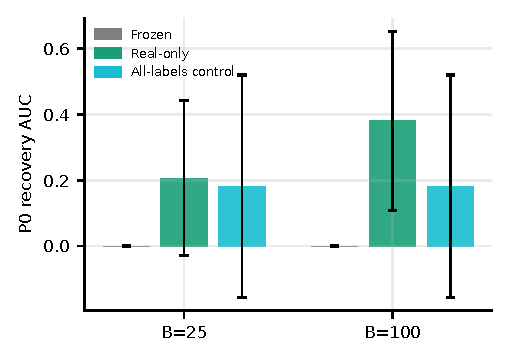
\includegraphics[width=0.78\columnwidth]{figures/fig_p0.pdf}
\caption{P0 recovery AUC (mean, 95\% $t$-interval, $n{=}5$). The all-labels control is \emph{not} better than budgeted real-only adaptation at $B{=}100$: more labels produce candidates the safety gate cannot clear.}\label{fig:p0}\end{figure}
\begin{table}[t]\centering\caption{P0, $B{=}100$: per-seed window cells.}\label{tab:p0}\footnotesize
\begin{tabular}{lcccl}
\toprule
Seed & Cells & Assessable & GO cells & GO class \\
\midrule
0 & 9 & 8 & 8 & PortScan \\
1 & 9 & 9 & 5 & PortScan \\
2 & 9 & 8 & 3 & PortScan \\
3 & 9 & 9 & 4 & PortScan \\
4 & 9 & 9 & 7 & PortScan \\
\bottomrule
\end{tabular}
\end{table}

\subsection{P1: the preregistered test fails}
Table~\ref{tab:hyp} and Fig.~\ref{fig:forest} show the fixed sequence. H2 is not rejected: the paired improvement of CTRL+SMOTE over real-only adaptation is \HTwoMean{} [\HTwoLo, \HTwoHi]; it is \emph{exactly} zero in all ten seeds, because the controller never changes the candidate (below). The sequence stops, the learned-generator stage (P2) is not run, and CTRL+SMOTE is non-inferior to the fixed doses only trivially. H4 is ``safe by inaction'': \hFourBreaches{} envelope breaches, synthetic candidates promoted in \hFourSeeds{} of \nSeeds{} seeds. Fired reporting conditions: F2, F3a, F3b, F8 (degenerate controller).

\begin{table}[t]\centering\caption{Preregistered tests. Differences in \Rrec{}; $n{=}\nSeeds$ paired seeds.}\label{tab:hyp}\scriptsize
\resizebox{\columnwidth}{!}{\begin{tabular}{lcc}
\toprule
Test & Paired difference [95\% CI] & Result \\
\midrule
H2 Ctrl+SMOTE $-$ real-only & 0.000 [0.000, 0.000] & not rejected \\
H3a Ctrl+SMOTE $-$ Ctrl+dup. & 0.000 [0.000, 0.000] & n/a (sequence stopped) \\
H3b Ctrl+SMOTE $-$ Ctrl+thr. & 0.000 [0.000, 0.000] & n/a (sequence stopped) \\
H5 Ctrl+SMOTE $-$ Fixed SMOTE $\rho{=}1$ & 0.000 [-0.002, 0.002] & n/a (sequence stopped) \\
H5 Ctrl+SMOTE $-$ Fixed SMOTE $\rho{=}4$ & -0.001 [-0.004, 0.001] & n/a (sequence stopped) \\
\bottomrule
\end{tabular}
}\end{table}
\begin{figure}[t]\centering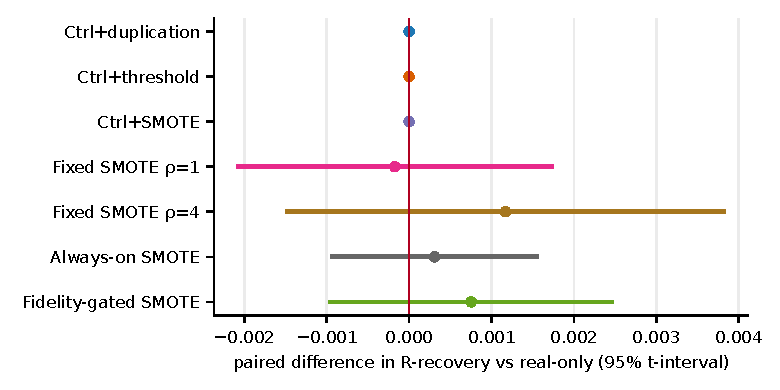
\includegraphics[width=\columnwidth]{figures/fig_forest.pdf}
\caption{Paired difference in deployed \Rrec{} against real-only adaptation. Every arm is within noise of real-only; the controller arms are identical to it.}\label{fig:forest}\end{figure}
\begin{table}[t]\centering\caption{Main arms (deployed \Rrec{}, mean [95\% CI]), promotions (synthetic/real-only candidate), rollbacks, held-out envelope breaches (point estimates on $S_{\mathrm{report}}$), CPU minutes.}\label{tab:arms}\scriptsize
\resizebox{\columnwidth}{!}{\begin{tabular}{lcccrr}
\toprule
Arm & R-recovery [95\% CI] & Promoted (syn/real) & Rollbacks & Breaches & Min \\
\midrule
Real-only & 0.623 [0.387, 0.859] & 0/14 & 0 & 0 & 2.2 \\
Ctrl+duplication & 0.623 [0.387, 0.859] & 0/14 & 0 & 0 & 3.5 \\
Ctrl+threshold & 0.623 [0.387, 0.859] & 0/14 & 0 & 0 & 2.5 \\
Ctrl+SMOTE & 0.623 [0.387, 0.859] & 0/14 & 0 & 0 & 3.6 \\
Fixed SMOTE $\rho{=}1$ & 0.623 [0.387, 0.859] & 2/13 & 0 & 2 & 3.6 \\
Fixed SMOTE $\rho{=}4$ & 0.625 [0.388, 0.861] & 3/13 & 0 & 1 & 3.7 \\
Always-on SMOTE & 0.624 [0.387, 0.860] & 2/13 & 0 & 2 & 4.2 \\
Fidelity-gated SMOTE & 0.624 [0.388, 0.861] & 2/13 & 0 & 0 & 4.6 \\
\bottomrule
\end{tabular}
}\end{table}

\subsection{Why: the controller cannot certify a first step}
Over all seeds and windows the controller faced a need set in \eligibleRuns{} runs and accepted no step in \eligibleKzero{}
(Fig.~\ref{fig:stops}). For CTRL+SMOTE, \CandPosCtrlSmote{} of \CandCtrlSmote{} evaluated steps had a positive \emph{point} gain on the selection set (maximum \CandMaxPtCtrlSmote{}) but the largest \emph{lower bound} was \CandMaxLcbCtrlSmote{}; for duplication \CandPosCtrlRos{} point-positive, maximum bound \CandMaxLcbCtrlRos{}; for the threshold operator \CandPosCtrlThresh{} point-positive with maximum bound \CandMaxLcbCtrlThresh{}, below the step cost $\eta{=}0.02$. The first rung ($\rho{=}0.5$) adds a median of \CandMedRowsCtrlSmote{} synthetic rows; the selection set holds only on the order of a hundred to a few hundred labels of all classes, so a lower bound at level $\alpha/K_{\max}$ on so small a paired change cannot clear $\eta$. This is a statement about the frozen design at $B{=}100$, not a proof that no dose helps: the greedy search never reaches the larger doses that the fixed-dose arms test directly. The negative controls and every ablation that keeps the step test are therefore also identical to real-only adaptation (Table~\ref{tab:abl}; per-window decisions in Fig.~\ref{fig:grid}, recovery curves in Fig.~\ref{fig:curves}), so those controls cannot, by themselves, say anything about selectivity (F11 did not fire for the trivial reason that nothing was ever added).

\begin{figure}[t]\centering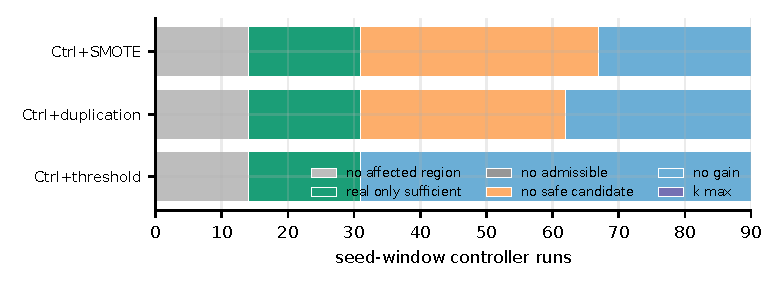
\includegraphics[width=\columnwidth]{figures/fig_stops.pdf}
\caption{Why the controller stopped, per seed-window.}\label{fig:stops}\end{figure}

\subsection{Candidate quality is not the bottleneck; certification is}
Fixed-dose SMOTE does build better candidates than real-only adaptation (Fig.~\ref{fig:cand}): $+\ShDiffFixedSmoteFourMean$ F1 at $\rho{=}4$ (CI [\ShDiffFixedSmoteFourLo, \ShDiffFixedSmoteFourHi]), $+\ShDiffFixedSmoteOneMean$ at $\rho{=}1$ and $+\ShDiffFidgateSmoteMean$ with the MMD pre-filter. These are exploratory descriptive contrasts, about one F1 point. Deployed, they vanish: $+\DepDiffFixedSmoteFourMean$ [\DepDiffFixedSmoteFourLo, \DepDiffFixedSmoteFourHi] at $\rho{=}4$ and $\DepDiffFixedSmoteOneMean$ at $\rho{=}1$. The oracle-dose reference (best rung chosen on the next window's reporting rows, never deployed) is only $+\ShDiffOracleDoseMean$ [\ShDiffOracleDoseLo, \ShDiffOracleDoseHi] above real-only candidates, so dose tuning has little headroom either. The gap that dominates everything is between what real-only adaptation \emph{could} deploy and what it does: candidates score \ShRealOnlyMean{} on the matched windows, the deployed model \RmRealOnlyMean{} (a gap of \gapRealOnly{}); for the all-labels control the gap is \ShRealOnlyAllLabelsMean{} versus \RmRealOnlyAllLabelsMean{}, and its deployed \Rrec{} (\RrRealOnlyAllLabelsMean) is \emph{below} the budgeted real-only arm. The gate's decisions for real-only adaptation were: \NRealOnlyPromoted{} promoted, \NRealOnlyEnvelopeInconclusive{} rejected because the envelope could not be shown safe, \NRealOnlyUtilityNoGain{} and \NRealOnlyUtilityInconclusive{} for no demonstrated gain, \NRealOnlyNoAffectedRegion{} with nothing to do (Fig.~\ref{fig:gate}). Of the \gbRejected{} real-only candidates rejected with a gate report, \gbUtilOkEnvFail{} had a demonstrated utility gain and failed only the safety envelope. The envelope criteria that failed were the stable-class macro-F1 on $S_{\mathrm{gate}}$ (\gbStableF{} windows) and the benign-FPR rise on $D_{\mathrm{gate}}$ (\gbFprCur{} windows; median \gbMedBenign{} benign gate rows, so one extra benign false positive moves the rate by \gbOneFp{}, above $\eps_{\mathrm{FPR}}{=}0.005$); the utility test failed in \gbUtil{} (exploratory counts; a window can fail several criteria). With abundant labels the benign-FPR criteria dominate instead (\gbAllFprCur{} and \gbAllFprStable{} of \gbAllRejected{} rejections, median \gbAllMedBenign{} benign gate rows): there the cost is a real false-positive increase, not sampling noise. Finally, in \seedsNeverDeployed{} of \nSeeds{} seeds (seeds \seedsNeverDeployedList) no model was ever certified, although their candidates reach 0.89--0.92.

\begin{figure}[t]\centering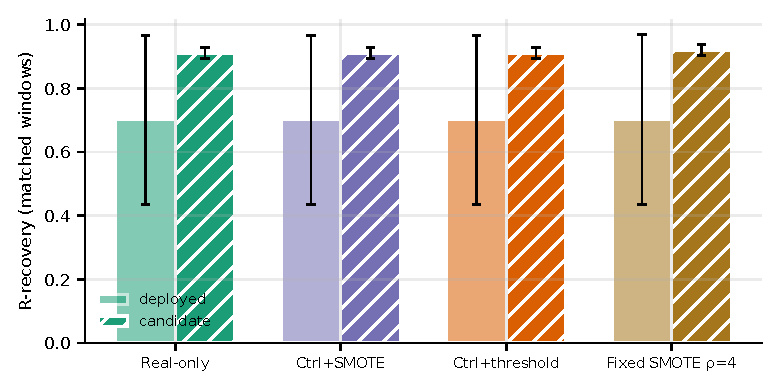
\includegraphics[width=\columnwidth]{figures/fig_candidate_vs_deployed.pdf}
\caption{Deployed model versus the candidate that would have been deployed, same windows. The shaded gap is value that exists but cannot be certified.}\label{fig:cand}\end{figure}
\begin{figure}[t]\centering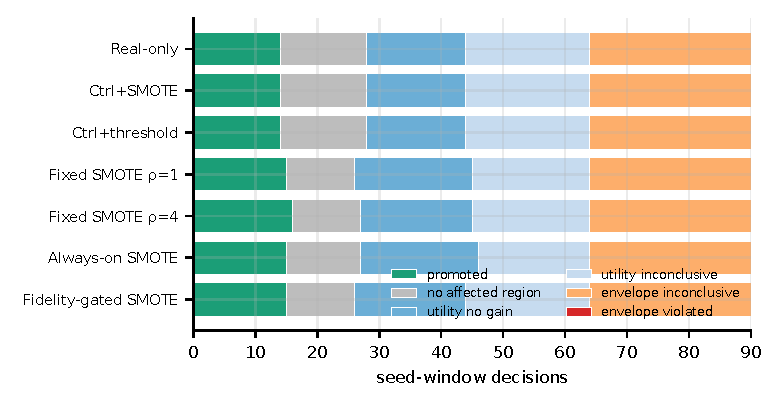
\includegraphics[width=\columnwidth]{figures/fig_gate_outcomes.pdf}
\caption{Final outcome per seed-window at the promotion gate. Amber: the envelope could not be shown safe.}\label{fig:gate}\end{figure}
\begin{figure}[t]\centering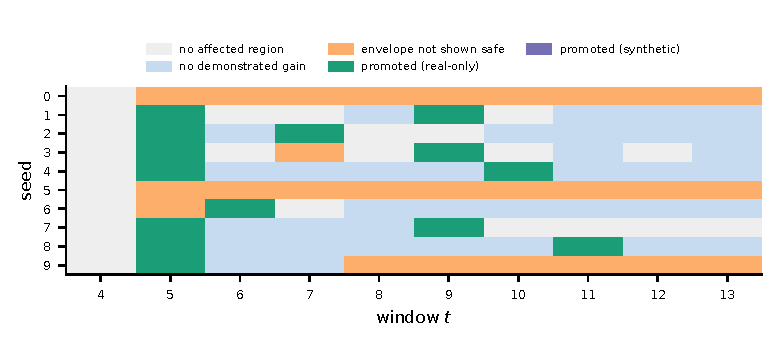
\includegraphics[width=\columnwidth]{figures/fig_decision_grid.pdf}
\caption{CTRL+SMOTE decisions for every seed and window (no synthetic candidate is ever promoted; Fig.~\ref{fig:gate} aggregates the gate's reasons).}\label{fig:grid}\end{figure}
\begin{figure}[t]\centering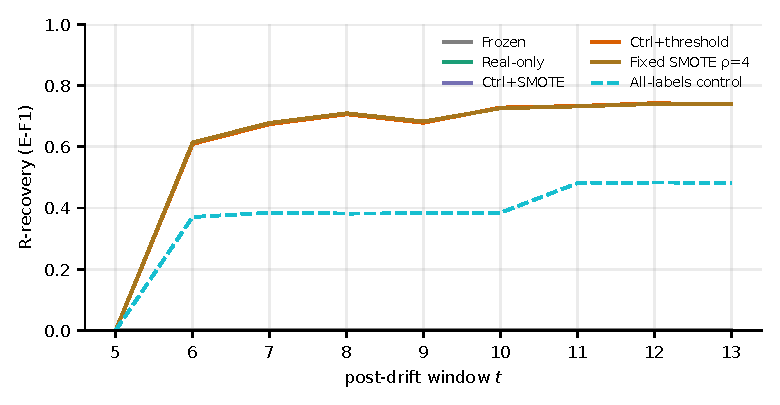
\includegraphics[width=\columnwidth]{figures/fig_curves.pdf}
\caption{R-recovery by post-drift window (mean over seeds, deployed model).}\label{fig:curves}\end{figure}

\subsection{Safety, canary and controls}
No promoted real-only model broke the held-out envelope (\BreachRealOnly{} breaches over \NonBaseRealOnly{} non-base windows). Promoted synthetic candidates did: \BreachFixedSmoteOne{}, \BreachFixedSmoteFour{}, \BreachAlwaysSmote{} and \BreachAblNoStepTest{} breach windows (point estimates on $S_{\mathrm{report}}$) for fixed $\rho{=}1$, fixed $\rho{=}4$, always-on SMOTE and the no-step-test ablation, from \StarFixedSmoteOne{}, \StarFixedSmoteFour{}, \StarAlwaysSmote{} and \StarAblNoStepTest{} star promotions, which indicates that a UCB gate on one sample is not a guarantee on a different held-out sample over many windows. The canary performed \ChkRealOnly{} checks for real-only adaptation and rolled back \RollRealOnly{}; there were no rollbacks in any arm. In the 30 pre-drift windows the controller returned an empty region every time (\probeNonempty{} non-empty), so it does nothing without drift. Pooling selection and gate sets (a winner's-curse check, never a method) promoted \RealAblPooled{} models versus \RealRealOnly{} and moved deployed \Rrec{} by $+\DepDiffAblPooledMean$ [\DepDiffAblPooledLo, \DepDiffAblPooledHi], i.e.\ a more permissive but double-dipping gate would look slightly better.

\begin{table}[t]\centering\caption{Controls, ablations and references (deployed \Rrec{}, paired difference against Ctrl+SMOTE for ablations and against real-only otherwise).}\label{tab:abl}\scriptsize
\resizebox{\columnwidth}{!}{\begin{tabular}{lcccc}
\toprule
Variant & R-recovery & Contrast & Paired diff. & Prom. (syn/real) \\
\midrule
no step test & 0.623 [0.387, 0.859] & vs Ctrl+SMOTE & 0.000 [0.000, 0.000] & 1/14 \\
no need test ($I{:=}A$) & 0.623 [0.387, 0.859] & vs Ctrl+SMOTE & 0.000 [0.000, 0.000] & 0/14 \\
no step safety & 0.623 [0.387, 0.859] & vs Ctrl+SMOTE & 0.000 [0.000, 0.000] & 0/14 \\
$K_{\max}{=}1$ & 0.623 [0.387, 0.859] & vs Ctrl+SMOTE & 0.000 [0.000, 0.000] & 0/14 \\
+MMD pre-filter & 0.623 [0.387, 0.859] & vs Ctrl+SMOTE & 0.000 [0.000, 0.000] & 0/14 \\
pooled sel/gate & 0.628 [0.390, 0.866] & vs Ctrl+SMOTE & 0.005 [-0.000, 0.009] & 0/17 \\
ctrl, no canary & 0.623 [0.387, 0.859] & vs Ctrl+SMOTE & 0.000 [0.000, 0.000] & 0/14 \\
real-only, no canary & 0.623 [0.387, 0.859] & vs Ctrl+SMOTE & 0.000 [0.000, 0.000] & 0/14 \\
NC1 wrong-class rows & 0.623 [0.387, 0.859] & vs real-only & 0.000 [0.000, 0.000] & 0/14 \\
NC2 Gaussian & 0.623 [0.387, 0.859] & vs real-only & 0.000 [0.000, 0.000] & 0/14 \\
NC3 shuffled & 0.623 [0.387, 0.859] & vs real-only & 0.000 [0.000, 0.000] & 0/14 \\
NC4 placebo (DDoS) & 0.623 [0.387, 0.859] & vs real-only & 0.000 [0.000, 0.000] & 0/14 \\
All-labels control & 0.372 [0.070, 0.674] & vs real-only & -0.251 [-0.732, 0.230] & 0/5 \\
Oracle dose (ref.) & 0.000 [0.000, 0.000] & vs real-only & -0.623 [-0.859, -0.387] & 0/0 \\
\bottomrule
\end{tabular}
}\end{table}

\subsection{Ambiguity and scenario S2}
Contradictory labels do not explain the residual. For real-only candidates PortScan recall is \recallAll{} over \nGoRows{} rows, \recallClean{} on non-ambiguous rows and \recallAmbig{} on the \shareAmbig\% ambiguous rows; the deficiency on clean rows is far above $\eps_{\mathrm{def}}$ (F9 not fired). The P1 run is a replay of P0 where they overlap: with the canary off, real-only adaptation reproduces the frozen P0 REAL\_ONLY decision, reason and reporting confusion cells at every window of seeds 0--4.

Scenario S2 was run only through its P0 gate under the unchanged rules: outcome \sTwoOutcome{} (\sTwoScope), valid, assessable in \sTwoAssessSeeds{} of 5 seeds at both budgets and with \sTwoGoCells{} GO cells. Repairable classes are the DoS family (\sTwoR). Recovery AUC of real-only adaptation is \sTwoAucBOneZeroZeroRealOnly{} at $B{=}100$ against \sTwoAucBOneZeroZeroRealOnlyAllLabels{} for the all-labels control, yet no residual deficiency is \emph{certifiable} in candidates, again pointing at deployment rather than candidate quality. By the preregistered rule P3 is not run.

\section{Discussion}
\textbf{What the evidence supports.} (i) Under a leak-free protocol and a realistic label budget there is real but narrow room for intervention (one class, ambiguity-qualified). (ii) A sequential controller that must prove each dose step with a confidence bound does not move off real-only adaptation at $B{=}100$. (iii) Synthetic rows built with a fixed dose improve held-out candidate quality by about a point of F1, a gain that is not deployable. (iv) The dominant loss is the distance between candidate quality and certified quality. \textbf{What it does not support.} It does not show that synthetic augmentation is useless in general, that a different learner, larger label budget, a different step/gate design, or a learned generator cannot do better, or anything about live SDN deployment. The oracle-dose and always-on arms suggest the headroom for \emph{better doses} is small here, but the controller's no-op result is conditional on the frozen constants.

\textbf{Implication.} For this class of systems the practical lever is the evidence budget of the safety test (more benign gate labels, pooled or sequential evidence, a less conservative per-quantity bound chosen \emph{before} looking), not the sophistication of the generator. A preregistered follow-up would vary the evidence rather than the generator; we state it as future work and do not run it, because changing the frozen constants after seeing this result would void the preregistration.

\section{Threats to Validity}
\emph{One effective class.} Only PortScan produces a GO; positive results would concern it alone. \emph{Analysis-time set $R$.} It is derived from the all-labels control and used by the endpoint, not by any arm. \emph{Post-hoc choices.} The incremental step filter and the $R$-restricted endpoint were fixed after reading P0 descriptives and before any P1 data; they are recorded with their reason. \emph{Controls.} Because the controller never adds rows, the negative controls and most ablations are vacuous; selectivity is untested. \emph{Single learner, oracle trigger, one-window delay, shuffled stationary drift day.} KS-triggered operation and time-ordered replay are not evaluated. \emph{Exploratory contrasts} (candidate quality, oracle dose, breaches) are descriptive and not corrected for multiplicity. \emph{Held-out breaches} are point estimates on one 20k-row sample. \emph{Residual duplicates.} Identical flows can recur across windows; they are group-disjoint from reporting rows but not from other learning rows, so the canary may see duplicates of training rows. \emph{Nothing here ran on a live network}; 39 of 52 deployment features are defaulted by the OpenFlow mapper.

\section{Reproducibility}
All artifacts are in \texttt{results/} with SHA-256 digests: \texttt{intervention\_p0\_S1\_*.json} (frozen P0), \texttt{results/p1/intervention\_p1\_S1\_B100\_seed*.json} (one file per seed, with the rules hash \rulesHash, criteria digest, parameter digest and per-file code hashes), \texttt{intervention\_p1\_S1\_B100\_summary.json}, \texttt{intervention\_p1\_S1\_B100\_decisions.json} and \texttt{intervention\_p0\_S2\_*.json}. Commands from the repository root:
\texttt{python -m proteus.intervention.cache build};
\texttt{python -m proteus.intervention.p0} (P0, frozen);
\texttt{python -m proteus.intervention.p1} (campaign);
\texttt{python -m proteus.intervention.analyze\_p1};
\texttt{python -m proteus.intervention.p0\_s2};
\texttt{python paper/p1/make\_assets.py} and \texttt{latexmk -pdf main.tex} in \texttt{paper/p1}. Every figure, table and number in this paper is generated from those files. The campaign ran from the base commit \gitSha{} with an uncommitted working tree (committed afterwards); the per-file code hashes identify the exact code.

\section{Conclusion}
We built and preregistered the most direct version of ``feedback-controlled synthetic intervention'': decide class and dose from observed recovery value inside a safety envelope. Against a fair real-only baseline it did nothing, because with about a hundred labels per window the evidence needed to certify even a small synthetic dose does not exist. The same evidence limit throttles real-only adaptation itself, which deploys only about \RmRealOnlyMean{} of the \ShRealOnlyMean{} its candidates reach. The result is a negative one about synthetic data in this regime and a positive one about where to look next: the certification step.

\bibliographystyle{IEEEtran}
\bibliography{refs}
\end{document}
